\documentclass{standalone}
\usepackage{standtikz}
\begin{document}
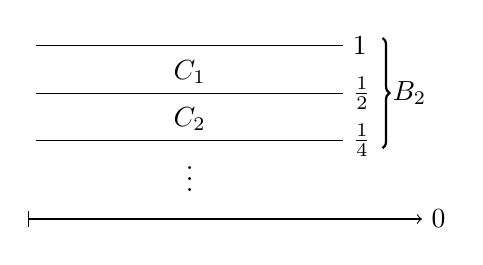
\begin{tikzpicture}[decoration=brace]
  \draw[|->,black] (0,0)--(5,0) node [anchor=west,pos=1]{0};
  \draw[black] (0.1,1)--(4,1) node [anchor=west,pos=1]{$\frac{1}{4}$}node[midway,anchor=south]{$C_2$} node[midway,anchor=north]{$\vdots$};
  \draw[black] (0.1,1.6)--(4,1.6) node [anchor=west,pos=1]{$\frac{1}{2}$} node[midway,anchor=south]{$C_1$};
  \draw[black] (0.1,2.2)--(4,2.2) node [anchor=west,pos=1]{1};
  \draw[black,decorate,thick] (4.5,2.3)--(4.5,0.9) node[anchor=west,midway]{$B_2$};
\end{tikzpicture}
\end{document}